\documentclass[11pt]{article}
% Named course report. Use review mode only if the course requests anonymity.
\usepackage[preprint]{acl}
\usepackage{times}
\usepackage{latexsym}
\usepackage[T1]{fontenc}
\usepackage[utf8]{inputenc}
\usepackage{microtype}
\usepackage{graphicx}
\usepackage{booktabs}
\usepackage{amsmath}
\usepackage{xcolor}
\usepackage{tikz}
\usetikzlibrary{arrows.meta,positioning}

\title{Explanation Budgets for Small Multilingual Language Models:\\A Preliminary MGSM Study}
\author{Mukthish B \quad Sushma Gandham \quad Aryan Srivastava \quad Praptipriya Phukon \\ BITS Pilani}

\begin{document}
\maketitle

\begin{abstract}
How much visible explanation should a small multilingual language model produce? We compare 0, 2, 4, 8, and 16 requested steps on parallel English, Bengali, and Telugu MGSM questions using frozen Qwen3 1.7B and 4B checkpoints. A local NF4 pilot completes 2,300 responses on 50 matched development IDs, representing 20\% of the planned evaluation grid. For 4B English native explanations, four to sixteen steps reduces numerical accuracy from 86\% to 74\%, with an exploratory paired 95\% interval of [$-24$, $-2$] percentage points, while mean generated tokens rise from 118.9 to 318.6. Four of seven lost correct answers have missing answer markers at sixteen steps, qualifying interpretation of the decline. Other budget and pivot effects vary by language and checkpoint. Independent numerical review of ten diagnostic cases agrees with benchmark answers and scoring decisions. We provide reproducible audits and observable error evidence, keeping every response in the accuracy denominator. Held-out budget routing is future work. The pilot does not establish a reasoning-capacity cliff.
\end{abstract}

\section{Introduction}
Mathematical word problems require language understanding and correct calculation. GSM8K \citep{cobbe2021gsm8k} and MGSM \citep{shi2023mgsm} provide benchmarks. Chain-of-thought and zero-shot prompting request explanations \citep{wei2022cot,kojima2022zeroshot}; self-consistency, least-to-most, and PAL instead aggregate paths, decompose problems, or execute programs \citep{wang2023selfconsistency,zhou2023leasttomost,gao2023pal}. We study the simpler intervention of changing requested explanation length in one response.

Multilingual evaluation \citep{hu2020xtreme}, instruction tuning \citep{mcot2024}, English reasoning \citep{linguafranca2026}, and language-consistency training \citep{lang2026} motivate comparing explanation languages. TALE addresses token efficiency \citep{han2025tale}, while compositionality and faithfulness studies caution against reading explanation text as proof of correct reasoning \citep{press2023compositionality,turpin2023faithfulness}. These approaches leave practical questions about requested step budgets for frozen small multilingual checkpoints.

We compare Qwen3 1.7B and 4B \citep{qwen2025} on the same English, Bengali, and Telugu problems. Native and English-pivot requests share sampling settings and an output ceiling. These experimental contributions do not establish a new reasoning algorithm or a capacity cliff.

\paragraph{Objectives.}
RQ1 measures accuracy across five requested step budgets. RQ2 compares native and English-pivot explanations across languages and checkpoints. A future RQ3 will test question-dependent routing for accuracy and token cost.

\paragraph{Contributions.}
The completed pilot provides:
\begin{itemize}
\item A matched sweep of five visible explanation budgets and two explanation-language strategies.
\item A reproducible 2,300-response local NF4 experiment with independently reconciled numerical scores.
\item Paired token-cost and formatting diagnostics, supplemented by ten human numerical checks.
\end{itemize}

\section{Related Work}
\subsection{Reasoning prompts and efficiency}
Chain-of-thought \citep{wei2022cot} and zero-shot prompting \citep{kojima2022zeroshot} request explanations. Self-consistency \citep{wang2023selfconsistency} votes over paths; least-to-most \citep{zhou2023leasttomost} solves subproblems; PAL \citep{gao2023pal} executes programs. Compositionality \citep{press2023compositionality} and faithfulness \citep{turpin2023faithfulness} studies caution against equating plausible text with correct reasoning. TALE \citep{han2025tale} addresses token efficiency. We sweep requested step counts in a fixed multilingual setup and record actual tokens.

\subsection{Multilingual reasoning}
XTREME \citep{hu2020xtreme} evaluates cross-lingual tasks; MGSM \citep{shi2023mgsm} supplies parallel math questions. mCoT \citep{mcot2024} uses multilingual instruction tuning. Recent work studies English reasoning \citep{linguafranca2026} and trains for reasoning quality and language consistency \citep{lang2026}. We compare frozen small checkpoints without fine-tuning. This differs from training-based approaches without implying wholly new multilingual routing.

\section{Methodology}
\subsection{Matched explanation-length intervention}
Figure~\ref{fig:system} separates development decisions from held-out evaluation. Each question is processed independently. The common English instruction requests native-language explanations, or English explanations for an Indic question, followed by a brief answer in the question's language and a common numerical marker. Direct-answer prompts request no explanation. Built-in Qwen thinking is disabled for every condition; all conditions share the same output ceiling and sampling settings.

\begin{figure}[t]
\centering
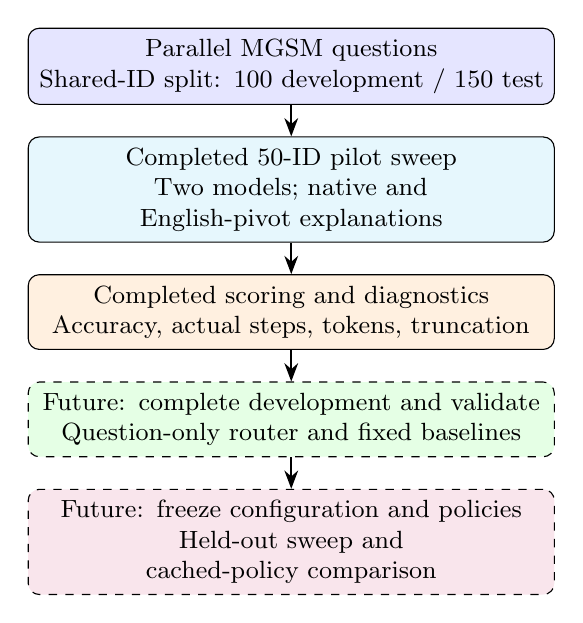
\begin{tikzpicture}[node distance=4mm, box/.style={draw, rounded corners, align=center, font=\small, text width=6.4cm, inner sep=4pt}, flow/.style={-{Stealth}, thick}]
\node[box,fill=blue!10] (data) {Parallel MGSM questions\\Shared-ID split: 100 development / 150 test};
\node[box,fill=cyan!10,below=of data] (sweep) {Completed 50-ID pilot sweep\\Two models; native and English-pivot explanations};
\node[box,fill=orange!12,below=of sweep] (score) {Completed scoring and diagnostics\\Accuracy, actual steps, tokens, truncation};
\node[box,dashed,fill=green!10,below=of score] (router) {Future: complete development and validate\\Question-only router and fixed baselines};
\node[box,dashed,fill=purple!10,below=of router] (test) {Future: freeze configuration and policies\\Held-out sweep and cached-policy comparison};
\draw[flow] (data) -- (sweep);
\draw[flow] (sweep) -- (score);
\draw[flow] (score) -- (router);
\draw[flow] (router) -- (test);
\end{tikzpicture}
\caption{Study workflow, separating the completed pilot from future routing and test stages (dashed boxes). Held-out outputs do not inform development; test inference requires a development freeze.}
\label{fig:system}
\end{figure}

\section{Experimental Setup}
\subsection{Data and models}
We use parallel MGSM \citep{shi2023mgsm}, derived from GSM8K \citep{cobbe2021gsm8k}. English, Bengali, and Telugu each have 250 rows: 750 records across 250 shared IDs. Source-row alignment and normalized numerical gold agreement are checked for every ID; neither proves translation fidelity. Pinned dataset and model revisions are supplied with the package.

Python's \texttt{random.Random(42)} shuffles shared IDs into 100 development and 150 held-out IDs. All translations share assignments. The first ten and 50 development IDs form nested smoke and pilot subsets; completed responses are reused. The pilot has 1,150 responses per model and 50 per condition. No held-out outputs exist.

\begin{table}[t]
\centering
\begin{tabular}{lrr}
\toprule
Response cohort & Planned & Completed \\
\midrule
Pilot (50 IDs) & 2,300 & 2,300 \\
Development & 4,600 & 2,300 \\
Held out & 6,900 & 0 \\
Full study & 11,500 & 2,300 \\
\bottomrule
\end{tabular}
\caption{Response coverage; rows are not additive. Each model/problem has 15 native and eight Indic English-pivot conditions; direct-answer pivots are omitted. The pilot completes 50 observations in each of 46 cells: 1,150 responses per model and 20\% of the full grid.}
\label{tab:grid}
\end{table}

\begin{figure*}[!t]
\centering
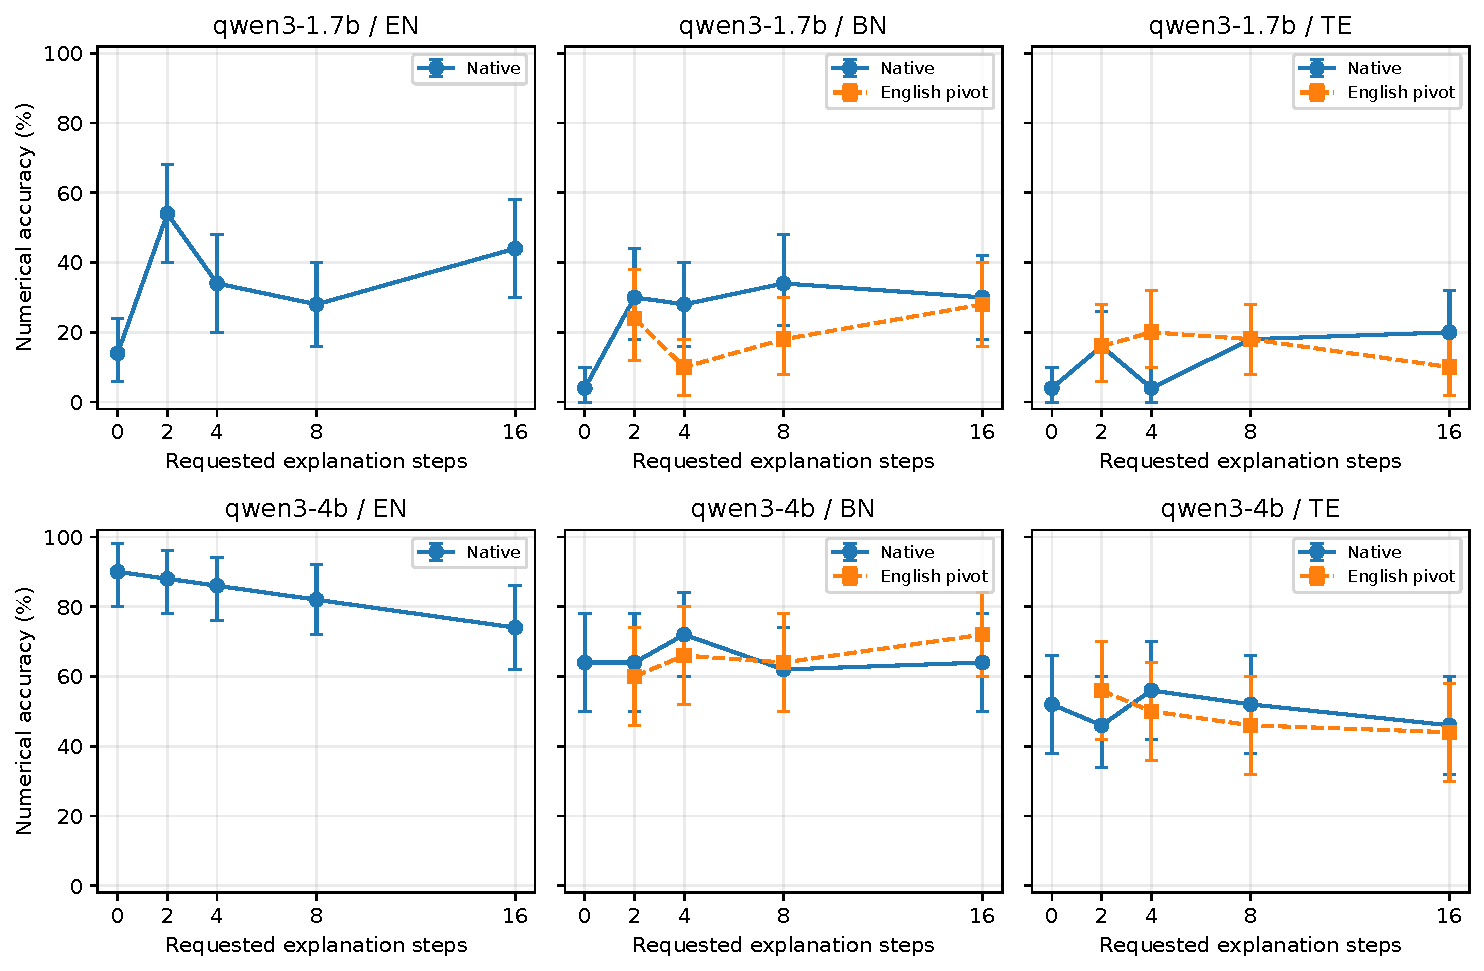
\includegraphics[width=\textwidth]{figures/pilot_accuracy_curves.pdf}
\caption{Numerical accuracy on 50 matched development IDs per condition. Rows are checkpoints and columns are question languages. Solid lines use native explanations; dashed lines use English pivots. Budgets request visible numbered steps. Error bars are exploratory 95\% shared-ID bootstrap intervals (2,000 resamples, seed 42); no multiplicity-adjusted significance is claimed.}
\label{fig:pilot-curves}
\end{figure*}

\begin{table*}[t]
\centering
\small
\setlength{\tabcolsep}{4pt}
\begin{tabular}{llrrrrrr}
\toprule
Model & Language & \shortstack{Accuracy\\(\%)} & \shortstack{Mean\\tokens} & \shortstack{Mean\\steps} & \shortstack{Count match\\(\%)} & \shortstack{Parse fail\\(\%)} & \shortstack{Truncated\\(\%)} \\
\midrule
Qwen3-1.7b & EN & 34$\to$44 & 97.1$\to$167.1 & 3.8$\to$7.7 & 84$\to$10 & 42$\to$34 & 0$\to$0 \\
Qwen3-1.7b & BN & 28$\to$30 & 281.6$\to$1000.2 & 4.0$\to$15.5 & 98$\to$64 & 16$\to$10 & 0$\to$6 \\
Qwen3-1.7b & TE & 4$\to$20 & 740.3$\to$1368.3 & 3.8$\to$13.9 & 92$\to$78 & 26$\to$12 & 10$\to$8 \\
Qwen3-4b & EN & 86$\to$74 & 118.9$\to$318.6 & 4.0$\to$15.9 & 98$\to$98 & 2$\to$10 & 0$\to$0 \\
Qwen3-4b & BN & 72$\to$64 & 319.1$\to$849.4 & 4.0$\to$16.0 & 98$\to$100 & 2$\to$0 & 0$\to$0 \\
Qwen3-4b & TE & 56$\to$46 & 698.8$\to$1652.3 & 3.9$\to$14.5 & 96$\to$88 & 6$\to$12 & 6$\to$12 \\
\bottomrule
\end{tabular}
\caption{Native four- to sixteen-step comparisons on the same 50 development IDs per row. Arrows show four-step then sixteen-step values. Accuracy retains parse failures and truncated outputs. Steps are mean numbered-line counts; count match does not establish semantic compliance.}
\label{tab:pilot-native}
\end{table*}


\subsection{Metrics, baselines, and implementation}
Numerical exact match requires one standalone \texttt{FINAL\_ANSWER:} marker and a finite decimal number. The study-specific parser normalizes Unicode digits, signs, valid western/Indian comma grouping, and equivalent decimal forms. Missing/duplicate markers, units, fractions, or invalid payloads fail parsing and count as incorrect. Last-line placement is requested but not required by the scorer. Every generated response, including parsing failures and truncation, stays in the denominator.

Diagnostics record tokens, numbered-line counts and compliance, parsing, truncation, repetition, and scripts within numbered lines. Counts and scripts do not establish semantic quality. Infrastructure failures are logged separately.

A separate audit reconciles all scores, tables, and paired intervals. Ten human numerical checks agree with benchmark answers and scoring. The Appendix supplies audit details, exact prompts, runtime versions, and future baselines.

Local inference uses an RTX 4060 Laptop GPU (8 GB), NF4 double quantization and FP16 compute. Batch size is one; temperature is 0.7, top-p 0.8, top-k 20, and the cap is 4,096 new tokens. Seeds, timing, memory, and termination are logged.

\section{Results and Discussion}
\subsection{RQ1: accuracy across explanation budgets}
Figure~\ref{fig:pilot-curves} shows the complete pilot curves. Table~\ref{tab:pilot-native} compares native four- and sixteen-step requests; the source package contains all 46 condition summaries and 26 prespecified contrasts.



For the 4B checkpoint on English questions, native four- to sixteen-step requests change accuracy from 43/50 (86\%) to 37/50 (74\%): $-12$ percentage points, exploratory paired 95\% interval [$-24$, $-2$]. Mean generated tokens increase from 118.9 to 318.6. Numbered-line count matches the request in 49/50 responses at both budgets, and neither condition is truncated. The paired outcomes include seven correct-to-incorrect transitions and one incorrect-to-correct transition. Four of the seven losses have missing final-answer markers at sixteen steps; parse failures increase from 1/50 to 5/50. These format associations qualify interpretation of the score decline without establishing its cause or a reasoning-capacity cliff. All 50 IDs remain in the primary comparison.

The 1.7B English native curve is nonmonotone (14\%, 54\%, 34\%, 28\%, 44\% at 0/2/4/8/16 requested steps). Its sixteen-minus-four difference is $+10$ points, interval [$-8$, $26.05$]. At sixteen steps, numbered-count compliance is only 10\%, versus 84\% at four steps. Requested length therefore cannot be equated with actual explanation length.

Prespecified contrasts compare native 16-minus-4, Indic/English differences in that effect, and pivot-minus-native. Intervals use the shared-ID bootstrap in Figure~\ref{fig:pilot-curves}.

\subsection{RQ2: language, pivot, and model comparisons}
Native sixteen-minus-four differences for EN/BN/TE are $+10/+2/+16$ percentage points for 1.7B and $-12/-8/-10$ for 4B. All four Indic-minus-English difference-in-effect intervals include zero, so the pilot does not establish a stronger Indic decline. The 4B checkpoint has descriptively higher accuracy in every matched condition, but checkpoint differences cannot be attributed solely to parameter count.

English pivot has no uniform advantage. At four steps, pivot-minus-native accuracy for 1.7B is $-18$ points on Bengali questions (interval [$-30$, $-6$]) and $+16$ on Telugu ([$4$, $28$]). These examples are exploratory; all 26 comparisons are exported to avoid selective reporting. Parsing, truncation, token cost, and numbered counts remain visible. Script diagnostics do not establish native-language fluency or semantic compliance; held-out validation is future work.

\subsection{Future RQ3: router and ablation}
Router training and ablation require the remaining development responses. Policies will be frozen before held-out inference and compared with fixed eight-step, global-best, and language-best budgets. No router benefit has been measured; implementation tests use synthetic fixtures only.

\subsection{Error analysis}
Seeded sampling across model and requested/question-language strata selects 40 incorrect responses (20 per model). Six fail parsing: four missing markers, one duplicate, and one invalid payload; none is truncated. The other 34 contain valid wrong answers. These counts cannot estimate overall error rates.

Of 24 English requests, 12 pass a response-text English-selection proxy, four are numeric-only, and eight primarily contain Indic script. This proxy differs from numbered-line script counts. Requested language and observable scripts do not establish fluency or semantic error categories.

\section{Conclusion}
The audited 2,300-response pilot shows that requested explanation length changes numerical scores and cost. For 4B English, accuracy falls from 86\% to 74\% between four and sixteen steps while mean tokens rise from 118.9 to 318.6. Four of seven lost correct answers have missing markers, so the decline alone cannot establish reduced reasoning capacity.

Language and pivot effects are heterogeneous, and requested steps need not match generated steps. The practical takeaway is to measure formatting and token cost alongside accuracy. Completing development, validating the router and its ablation, and freezing policies before held-out evaluation are future work.

\section*{Limitations}
The 50-ID pilot uses one NF4 setting and one sample per condition. Its development split prevents project leakage, not pretraining contamination. Checkpoints differ in more than parameter count; English instructions may affect native outputs. Scripts and numbered counts do not establish semantic quality, and native-language review requires suitable expertise. Results do not automatically generalize to full precision or held-out data. Diagnostic samples cannot estimate population error rates.

\section*{AI Use Statement}
AI assistance supported code, manuscript editing, source-linked checks, and observable diagnostic exports. It did not supply human review decisions or act as a semantic judge. Numerical, scoring-policy, figure, and manuscript checks were completed by human reviewers; recorded decisions and completion provenance accompany the results.

\clearpage
\bibliography{references}

\appendix
\section{Reproduction and Exact Prompts}
The source package includes original-data checksums, the shared-ID manifest, pinned model revisions, all generation settings, and command-line instructions. Table~\ref{tab:setup} summarizes the evaluation components. GPU responses are checkpointed by unique experiment ID. Future frozen router predictions will select cached held-out native outputs without additional model calls; no held-out outputs currently exist.

\begin{table}[t]
\centering
\begin{tabular}{p{1.9cm}p{4.6cm}}
\toprule
Component & Definition \\
\midrule
Data & MGSM \citep{shi2023mgsm}: 250 shared EN/BN/TE IDs; revision \texttt{3622039}. \\
Models & Qwen3 \citep{qwen2025}: 1.7B (\texttt{70d244c}) and 4B (\texttt{1cfa9a7}); both NF4. \\
Metric & Study-defined numerical exact match, including parse failures in the denominator. \\
Baselines & Future study-defined fixed eight-step, development-best global, and language-specific budgets. \\
\bottomrule
\end{tabular}
\caption{Dataset, checkpoints, metric, and future baseline definitions. Revision prefixes identify the full pinned hashes in the configuration; the baselines have no reported test scores.}
\label{tab:setup}
\end{table}

\subsection{Exact user-message templates}
The following templates reproduce \texttt{study/prompts.py}. Here $Q$ is the complete question text, $L_q$ is its language name (English, Bengali, or Telugu), $L_e$ is the requested explanation language, and $B$ is 2, 4, 8, or 16. Native requests set $L_e=L_q$; Indic pivots set $L_e$ to English. Substituting these values gives the complete messages supplied to the models. All instructions are in English, and no gold answer enters a prompt.

\paragraph{Direct answer ($B=0$).}
\begin{quote}\small\ttfamily
Solve the following mathematical word problem.\\
Give a direct answer. Do not show an explanation or numbered steps.\\
Give a brief final answer sentence in $L_q$.\\
Then put only the numerical answer on the last line in the exact format FINAL\_ANSWER: <number>. Do not include units or any other text on that last line.\\[0.5em]
Problem:\\
$Q$
\end{quote}

\paragraph{Numbered explanation ($B>0$).}
\begin{quote}\small\ttfamily
Solve the following mathematical word problem.\\
Explain the solution in $L_e$ using exactly $B$ numbered steps, with one step per line in the format '1. ...'. Do not add other explanation paragraphs.\\
Give a brief final answer sentence in $L_q$.\\
Then put only the numerical answer on the last line in the exact format FINAL\_ANSWER: <number>. Do not include units or any other text on that last line.\\[0.5em]
Problem:\\
$Q$
\end{quote}

Each prompt is a single user message rendered through the pinned tokenizer's chat template with \texttt{add\_generation\_prompt=True} and \texttt{enable\_thinking=False}. The grid export supplies every fully instantiated prompt without inference. A condition's seed is 42 plus the integer represented by the first eight hexadecimal digits of its experiment ID, modulo $2^{32}$.

\subsection{Question-only budget router}
We specify one decision tree per model with maximum depth three and minimum leaf size ten. Features are question language, character length, punctuation-based sentence count, and digit-based quantity count. Labels are the shortest development budget producing a correct answer. Questions with no successful budget are excluded from label fitting and their number is reported; evaluation still includes them. Five-fold validation groups every translation of a problem together. A tree without language supplies an ablation. No model answer or correct answer is available to the deployed selector.

\section{Local Runtime}
Local inference uses an NVIDIA RTX 4060 Laptop GPU with 8 GB VRAM, Python 3.12, PyTorch 2.8.0 with CUDA 12.6, Transformers 4.57.1, and bitsandbytes 0.48.1. Both checkpoints use NF4 weight quantization with double quantization and FP16 compute. Batch size is one, with temperature 0.7, top-p 0.8, top-k 20, and a common 4,096-new-token ceiling. Longest requested budgets run first within each problem block. Per-condition seeds, software versions, raw responses, latency, memory, and termination status are logged. Completed experiment IDs are reused across feasibility, smoke, and pilot stages; precision settings are not pooled.

\section{Audit and Planned Baselines}
A separate automated audit independently reconstructs dataset checksums and seed-42 splits, parses and scores the raw pilot responses without calling the production scorer, and reconciles scored records, summaries, and paired bootstrap intervals. It passes 169,916 checks with zero discrepancies. Its evidence is saved in the results package.

Independent human numerical review covers ten distinct questions, five per model: correct answers, valid wrong answers, and missing, duplicate, or invalid markers. Every case records a solution, benchmark/scoring agreement, reviewer, date, decision, and notes. All ten independent answers agree with the benchmark, and all scoring decisions are accepted. Other Person 1 checks were confirmed complete on October 13, 2026. This targeted review does not estimate population error rates or certify translation fidelity; semantic error classifications are not used in the reported analyses.

Router baselines are always eight steps, the development-best global budget per model, and the development-best language-specific budget per model. Fixed choices maximize training-fold accuracy, with shortest-budget tie breaking; they are refitted on full development before test evaluation. This efficiency comparison is motivated by budget-aware reasoning \citep{han2025tale}, but the baselines are policies defined in this study rather than imported implementations.

\section{Input-token Characterization}
\subsection{Completed input-token characterization}
We measured original question token counts on all 100 development IDs in the three languages, using each pinned tokenizer without model generation. Both checkpoints produced identical question token counts on this subset. Mean question lengths were 58.87 tokens in English, 249.44 in Bengali, and 375.67 in Telugu. Figure~\ref{fig:tokens} shows mean ratios computed within matched problem pairs: Bengali/English 4.21 (95\% bootstrap interval 4.10--4.32), and Telugu/English 6.36 (6.19--6.53).

\begin{figure}[t]
\centering
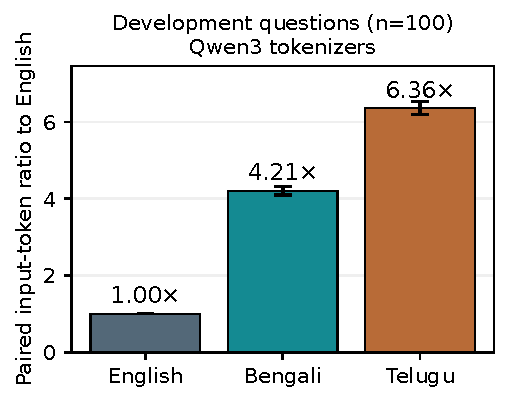
\includegraphics[width=\columnwidth]{figures/input_token_ratios.pdf}
\caption{Actual input-token ratios on 100 development problem IDs. Error bars resample matched IDs. These measurements describe tokenizer/input differences and do not establish an accuracy decline.}
\label{fig:tokens}
\end{figure}

This observation makes generated-token accounting particularly relevant: equal requested step counts need not imply equal textual cost across languages. Input-length differences alone cannot distinguish tokenization effects, translation length, language understanding, or reasoning capacity. No held-out questions were used in this characterization, and no gold answers were used to compute its statistics.

\end{document}

